\section{Overview}
	This chapter will explore the core engineering design of the DoodleBot. The implementation of these designs are covered in chapter ~\ref{ch:implementation}.

	The DoodleBot was designed to meet the Project Requirements, Project Scope and Performance Indicators introduced in Chapter ~\ref{ch:intro}. Figure ~\ref{fig:system} represents the overall architecture of the system. A key feature of the architecture is its modularity. Once appropriate data types are defined, each module of the system was able to be designed and tested in isolation. 
\begin{figure}[h]
\centering
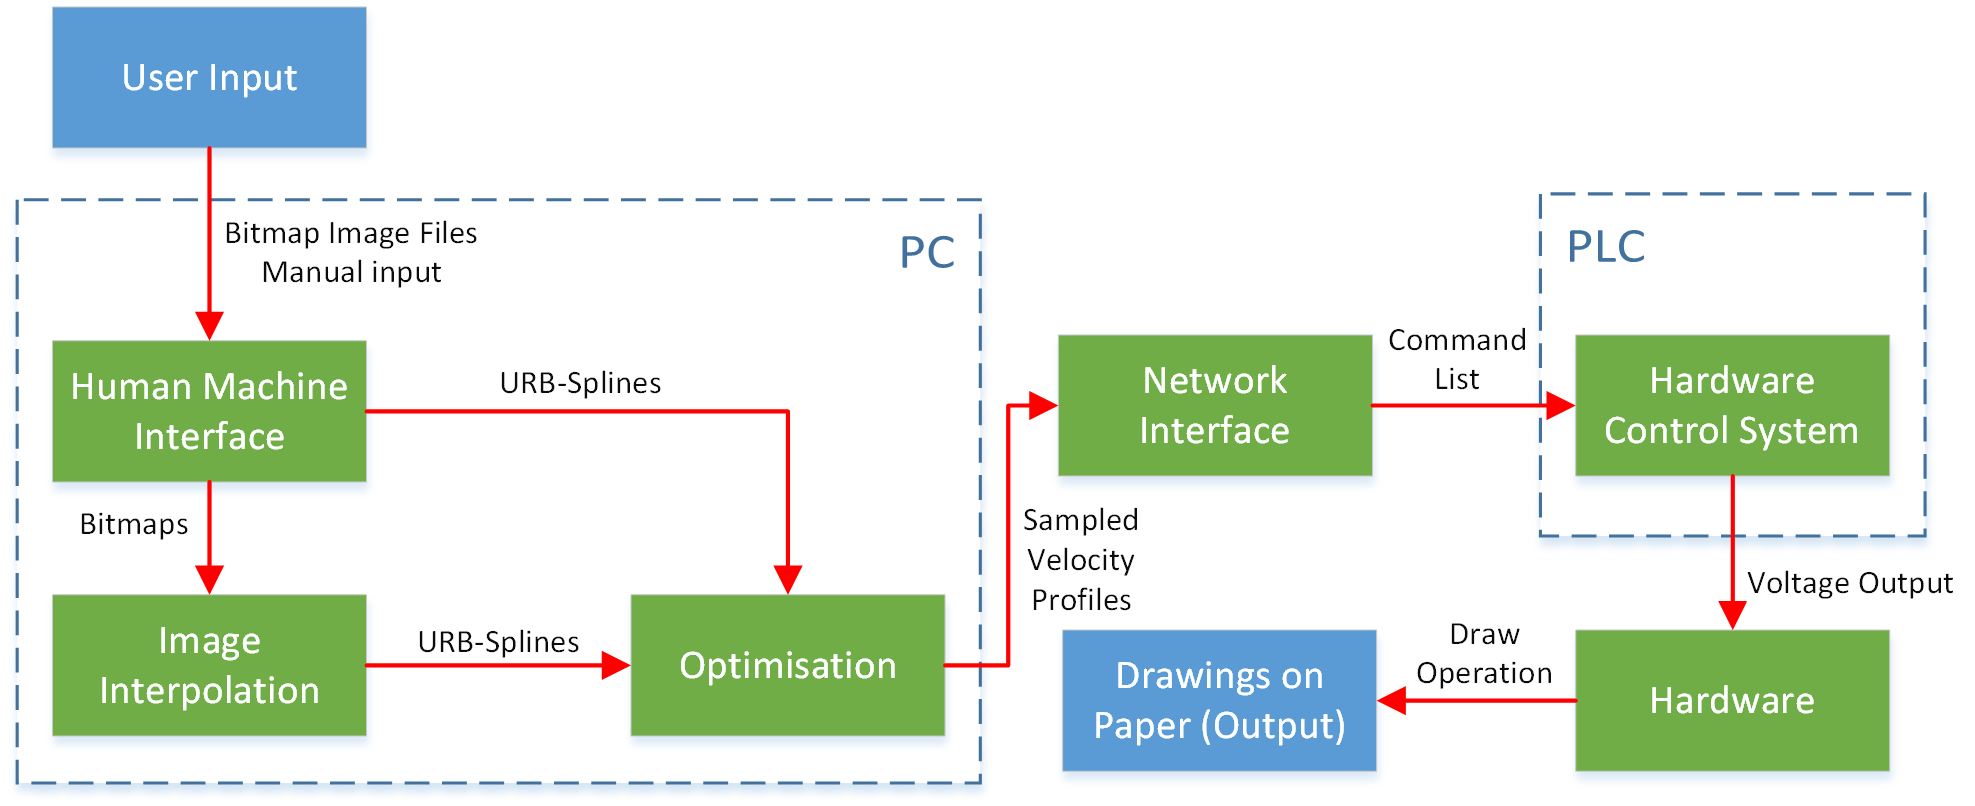
\includegraphics[width=0.9\textwidth]{figures/systemDesign/overview.png}
\caption{Modules and data flow of the DoodleBot system}
\label{fig:system}
\end{figure}

	\subsubsection*{Input}
		The requirements specify a user to be able to provide photos or images as input. The DoodleBot is designed to accept any bitmap format (including compressed formats such as JPEG or PNG). In addition to this, the DoodleBot provides the added functionality of allowing the user to define URB-Splines directly through the Human-Machine Interface Interface.
		
	\subsubsection*{Output}
		The required output is a representation of the input image to be drawn onto paper in a single colour via the DoodleBot mechanical hardware.
		
	\subsubsection*{Human-Machine Interface (HMI)} 
		The Human-Machine Interface (HMI) is the way a user interacts with the DoodleBot system and features a simple interface including the capability to provide both methods of input - selecting bitmap image files stored on the computer and constructing URB-Splines in an intuitive manner. Another feature is a way to control various parameters used in the optimisation process for testing and performance purposes.
		
	\subsubsection*{Quadratic URB-Splines}
		The quadratic Uniform Rational Basis Spline (URBS) was chosen as the data type into the optimisation section. It is a versatile way of representing various curves with very little data and is defined by mathematical equations that are convenient for the optimisation calculations. See Section ~\ref{sec:design-urbs}.
		
	\subsubsection*{Image to Spline Interpolation}
		The Image to spline interpolation module takes the bitmap image input to the DoodleBot and generates a representation of the input in terms of Quadratic URB-Splines for use by the optimisation module. This module is what generates the reference image that the hardware tries to ultimately draw onto the paper (ie, the output). See Section ~\ref{sec:design-interpolation}.
		
	\subsubsection*{Optimisation}
		Two of the performance indicators identified in Chapter ~\ref{ch:intro} were about how fast and how accurate the device can draw the image onto the output medium. The Optimisation module takes the input URB-Splines and generates velocity profiles (for use in the Hardware Control module) that are time optimal for given hardware constraints. See Section ~\ref{sec:design-optimisation}.

	\subsubsection*{Network Interface}
		One of the requirements of the project was to construct a network interface between the Programmable Logic Controller and the PC using an Ethernet connection. The network interface allows the sampled velocity profiles to be sent from the PC to PLC and involves software implemented on both devices. See section ~\ref{sec:network}.

	\subsubsection*{Hardware Control System}
		The Hardware Control System takes sampled velocity profiles for each axis and drives the two motors to match these profiles. It also controls the two-state control of the drawing head (Z-axis). See Section ~\ref{sec:design-control}.